\documentclass[conference]{IEEEtran}
\usepackage[UTF8, heading=true]{ctex}
\usepackage{amsmath,amssymb,amsfonts}
\usepackage{graphicx}
\usepackage{booktabs}
\usepackage{multirow}
\usepackage{array}
\usepackage{float}
\usepackage{cite}
\usepackage{hyperref}
\hypersetup{colorlinks=true,linkcolor=blue,citecolor=blue,urlcolor=blue}
\renewcommand{\figurename}{图}
\renewcommand{\tablename}{表}

\begin{document}

\title{物竞天择闭环：从Plaza讨论到最优Agent团队的完整演化路径\\
\large{Natural Selection Closed-Loop: From Plaza Deliberation to Optimal Agent Team Evolution}}

\author{\IEEEauthorblockN{AgentsGroup2026 研究团队}\IEEEauthorblockA{研究机构名称\\城市，国家\\Email: research@agentsgroup2026.org}}

\maketitle

\begin{abstract}
Large language model (LLM) agent teams currently rely on manually designed roles, yet the optimal team composition for any given task ecosystem remains unknown. This paper presents a complete closed-loop methodology that uses Darwinian natural selection to discover optimal multi-agent teams. The closed loop comprises five interconnected phases: (1) Plaza deliberation, where agents engage in ORID-structured discussion producing an ExecutionPlan and TaskHabitatContract; (2) skill extraction from the contract and discussion content to populate the skill universe; (3) natural selection evolution under ecological pressure via the EcoDrill engine, selecting agents through survival ticks $\tau$ as the sole native fitness metric; (4) validation and evaluation of emergent behaviors including collaboration rate, skill specialization, and dominant skill emergence; and (5) skill re-assignment, where evolution-identified dominant skills are written back to agent profiles, closing the loop. Experimental results from nine evolutionary runs spanning 45 agents demonstrate a significant inverted-U relationship between resource abundance and collaboration emergence ($R^2=0.43$, $p<0.01$), with collaboration peaking at moderate scarcity ($A\approx0.55$). Multi-generational mixed competition over nine generations uniquely produced five dominant skills, confirming that sustained temporal depth combined with cross-lineage recombination is necessary for skill heritability. Single-generation runs across different tournament formats showed no significant behavioral differences, reinforcing the primacy of ecological pressure over format in driving emergent team optimization. The full closed loop establishes natural selection as a principled methodology for discovering, rather than designing, optimal LLM agent team compositions.
\end{abstract}

\begin{IEEEkeywords}
多智能体系统，自然选择，团队优化，生态压力，技能进化，闭环系统，Plaza讨论，协作涌现
\end{IEEEkeywords}

\section{引言}

大语言模型驱动的多智能体系统在复杂任务的推理、规划和协作方面展现了显著潜力~\cite{wu2023autogen,park2023generative,hong2023metagpt,shinn2023reflexion}。当前主流框架（包括AutoGen、MetaGPT和CrewAI）均依赖人工工程师预先定义智能体的角色和技能边界——架构师负责架构审查，项目经理负责任务分解，运维工程师负责资源监控。这一静态角色分配范式面临一项根本性问题：对于任意给定的任务生态，\emph{最优的智能体团队组成是什么？}人工设计无法回答这个问题，因为它同时要求：(1) 对任务生态位的全局认知，(2) 对技能稀缺性的量化评估，以及 (3) 对团队内部协作经济性的跨角色平衡。这些需求超出了单个工程师的认知边界。

本文提出了一套完整的闭环方法论，利用达尔文自然选择原理来\emph{发现}而非\emph{设计}最优Agent团队。该闭环由五个相互连接的阶段组成，形成了一个自增强的适应性循环。

\emph{Plaza讨论}（Phase 1）作为闭环的起点：多智能体在一个结构化讨论空间中围绕特定任务展开审议，产出ExecutionPlan和TaskHabitatContract——后者明确定义了任务所需的生态位（niches）和技能需求。与自由对话或纯辩论范式不同，Plaza采用ORID四层递进结构（事实→风险→辩论→决策）和五指量表共识机制，确保讨论产出具有可操作的结构化和可追溯性~\cite{kaner2014facilitator}。

\emph{技能萃取}（Phase 2）将Plaza讨论的结构化输出转化为可量化的技能基因组：从Contract的demanded\_skills字段和Agent讨论内容中（通过NLP提取），抽取构成技能宇宙的基础元素。

\emph{演化选择}（Phase 3）是整个闭环的核心驱动力：技能基因组进入EcoDrill演化引擎，在代谢约束（HealthLedger）和生态压力参数（资源丰度$A$、捕食压力$P$、需求漂移$D$、生态位容量$K$）的共同作用下，通过自然选择筛选出适应度最高的个体。适应度的唯一度量是生存tick数$\tau$——不依赖人工评分，完全遵循达尔文框架的客观选择逻辑~\cite{darwin1859,lenski2003evolutionary}。

\emph{验证评估}（Phase 4）对演化结果进行多维度的量化分析：测量生存$\tau$、技能专精率（skill\%）、协作率（collab\%）和主导技能（dominant skill）的出现情况。

\emph{技能赋予}（Phase 5）将Phase 4确认的主导技能写回Agent配置文件，重新装备的Agent回到Plaza（Phase 1），携带进化积累的适应性知识进入下一轮任务讨论——完成环的闭合。

本研究的关键发现围绕三个方面展开。第一，资源丰度$A$对协作率具有显著的倒U型效应（$R^2=0.43$, $p<0.01$），协作在适度稀缺（$A\approx0.55$）处达到峰值，而在极端环境（严酷$A=0.35$或充沛$A=1.40$）下崩溃。这直接映射到Gause竞争排斥原理~\cite{gause1934struggle}和r/K选择理论。第二，单代跑次中赛事格式对智能体行为无显著影响，但多代混合竞争（9代，跨谱系重组）是唯一产生主导技能列表的条件——验证了Boyd和Richerson双继承理论中水平传播对垂直遗传的稳定化作用~\cite{boyd1985culture}。第三，生存$\tau$随生态压力呈单调梯度下降（充沛86 $>$ 压力67 $>$ 稀缺61 $>$ 严酷60），验证了代谢约束作为选择机制的工程有效性。这些发现共同建立了一条从多智能体讨论到技能发现、再到演化验证、最终回归闭环的完整通路，将自然选择确立为LLM Agent团队优化的原则性方法。

\section{闭环架构}

闭环系统由五个阶段组成，每个阶段解决团队优化问题的一个子维度，五个阶段的级联形成了从"任务定义"到"团队适配"的完整进化周期。

\subsection{Phase 1: Plaza讨论（Plaza Deliberation）}

Plaza是一个受多重理论启发的多Agent结构化讨论空间。智能体携带着各自的技能基因组进入Plaza，围坐于环状生态位布局中，围绕一个工程任务（如"AWS ES扩缩容方案"）展开审议。讨论的产出包括：(1) ExecutionPlan——后续执行的行动步骤，(2) TaskHabitatContract——明确定义了任务生态中的niche集合和每个niche所需的技能需求（demanded\_skills）。

与现有LLM讨论范式不同，Plaza的设计建立在三个经过实证验证的方法论之上。

\textbf{ORID四层递进结构。}讨论按ORID标准议程推进：事实层（Fact，5分钟）收集客观事实，风险层（Risk，5分钟）征集直觉性担忧，辩论层（Solution Debate，5分钟）采用TurQUaz冲突辩论模式~\cite{gungor2025turquaz}使对立方案进行多轮对抗，决策层（Decision，5分钟）通过五指量表达成共识~\cite{kaner2014facilitator}。四层总计20分钟的时间盒控制避免了讨论发散，保证了产出的浓度和可操作性。

\textbf{四Facilitator角色分工。}与单主持人模式不同，Plaza分配四个专门的Facilitator角色，各自控制一层议程：(1) Fact Keeper——只问"我们已知的客观事实是什么"，禁评解释与判断；(2) Emotion Reflector——只问"你的直觉告诉你最大的风险是什么"，禁驳他人的担忧；(3) Analyst——采用TurQUaz Council辩论模式的对抗性追问："如果假设不成立会发生什么"；(4) Decision Closer——通过五指量表量化每个Agent的承诺程度。这四个Facilitator永不对讨论内容进行引导——只控制流程，不介入观点——这是Plaza讨论区别于人类主持讨论的核心设计原则，其理论基础来自Khamsi等人~\cite{khamsi2024focus}的Focus Agent验证：LLM可以可靠地扮演纯流程Facilitator角色。

\textbf{五指量表共识机制。}结合Lippincott等人~\cite{lippincott2025fuzzy}的模糊共识建模，Plaza以连续型五指量表（1指=根本性反对，3指=有保留支持，5指=全力支持）替代了先前的关键词共识计数。这克服了两个先验问题：(1) 关键词级（agree/disagree）的二元化丢失了意图的粗细颗粒度，(2) 0.85硬阈值可能导致少数真诚异议被系统性地压制。当出现1指（根本性反对）时，Decision Closer追问"是什么让你不能接受"，聚焦该问题直到解决或记录为"有保留的共识"。

以上设计的核心目标不是产出"正确的答案"（MAD辩论的收敛目标），而是产出\emph{具有生态位结构定义的执行计划}——这是后续进化引擎所需的任务环境描述。

\subsection{Phase 2: Skill萃取（Skill Extraction）}

Plaza讨论结束后，系统从两个信息源中萃取技能需求。第一个来源是ExecutionPlan中的结构化niche定义：每个niche携带一个demanded\_skills列表，描述该生态位需要的核心能力。对于AWS运维任务，niche demanded\_skills包括{\texttt{aws\_es\_scaling\_orchestration}}、{\texttt{monitor\_alarms\_setup}}、{\texttt{cost\_ri\_advisor}}等。这些技能直接从合同解析，构成技能宇宙的骨架。

第二个来源是Plaza讨论的转录文本内容。通过NLP提取，系统识别Agent在对话中提及但未在合同中列出的技能需求——这捕获了讨论过程中涌现的知识，其中可能包含合同设计阶段未预见到的能力要求。例如，Agent在辩论过程中可能指出某个niche还需要{\texttt{interface\_definition}}或{\texttt{coverage\_analysis}}能力，这些需求通过讨论而非预定义产生。

两个来源的技能合并构成完整的技能宇宙（skill\_universe），作为Phase 3演化引擎的基因组池。

\subsection{Phase 3: 演化选择（Evolutionary Selection）}

EcoDrill是闭环系统的自然选择引擎。它接收Phase 2的技能宇宙和TaskHabitatContract，在代谢约束和生态压力下对Agent群体施加强度不同的选择压力，通过多代演化筛选出与任务生态位最匹配的Agent个体。每个Agent携带一个可变的技能基因组（Skill Genome，$S$）和协基因组（CollabGenome：分享/信号/跟随/挑剔），其生存状态由HealthLedger追踪。

\textbf{Fitness度量。}Agent的适应度由生存tick数$\tau$唯一决定——不使用任何人工评分、任务完成指标或外部奖励。$\tau$高意味着Agent在给定生态压力下维持了更长时间的正健康状态，这本质上等价于Darwin自然选择中的"存活至繁殖年龄"。与此并行，系统提供多种繁殖机制：技能基因组的垂直遗传（亲代crossover+mutation）、水平传播（盲学习、领养），并通过择偶机制（mate intention）将适应性差异转化为繁殖率差异。Darwin自然选择的四个必要条件——变异、遗传、生存竞争、差异繁殖——均在EcoDrill中满足~\cite{darwin1859,visscher2008heritability,gause1934struggle}，构成了一个逻辑完备的选择系统。

\textbf{生态压力参数。}EcoDrill的演化方向由四个参数控制：(1) 资源丰度$A$：低$A$代表资源稀缺，Agent需要更多tick才能达到目标的foraging成功；(2) 捕食压力$P$：独立于技能的随机失败概率，模拟外部事故；(3) 需求漂移$D$：任务需求在演化过程中的随机偏移；(4) 生态位容量$K$：每个niche的最大并发成功数。

\textbf{赛事模式。}为研究不同竞争结构对演化的影响，EcoDrill实现了四种赛事模式：

\begin{enumerate}
\item \textbf{Solo/Division}：Agent在自己的种群（pop）内独立觅食，种群间无交互。每个Agent仅与同种群内的个体竞争共享niche的位置。
\item \textbf{Confrontation}：两个种群（如aws-ops与build\_system）在同一个栖息地中竞争，但各自保留独立种群身份。Agent可跨越种群边界竞争niche。
\item \textbf{Mixed}：多种群完全混合竞争，跨谱系重组启用。这使得不同种群间的基因流成为可能——水平传播可以跨越种群边界传播技能基因。
\item \textbf{Habitat-Pressure}：在Solo/Division基础上叠加生态压力参数的精确控制（指定A、P、D、K的值）。
\end{enumerate}

\textbf{9-run实验矩阵。}为系统性地探索生态压力、赛事模式和任务域对Agent行为的影响，我们设计了9个跑次，跨两个任务域（AWS运维和Build系统）和多种压力配置。表~\ref{tab:config}展示了完整实验矩阵。

\begin{table}[t]
\centering
\caption{9-run演化实验矩阵}
\label{tab:config}
\setlength{\tabcolsep}{2pt}
\renewcommand{\arraystretch}{1.1}
\begin{tabular}{llcccc}
\toprule
跑次 & 任务域 & 赛事模式 & 代 & $A$ & $\tau$ \\
\midrule
aws-solo-division & AWS & Solo/Div & 1 & --- & 45 \\
build-solo-division & Build & Solo/Div & 2 & --- & 75 \\
aws+build-division & AWS+Build & Solo/Div & 1 & --- & 69 \\
aws+build-confrontation & AWS+Build & Confront & 1 & --- & 77 \\
aws+build-mixed & AWS+Build & Mixed & 9 & --- & 57 \\
habitat-pressure & AWS+Build & Solo/Div & 1 & 0.55 & 67 \\
habitat-scarce & AWS+Build & Solo/Div & 1 & 0.45 & 61 \\
habitat-harsh & AWS+Build & Solo/Div & 1 & 0.35 & 60 \\
habitat-abundant & AWS+Build & Solo/Div & 2 & 1.40 & 86 \\
\bottomrule
\end{tabular}
\end{table}

\textbf{关键发现：collab\%倒U型效应。}表~\ref{tab:regression}报告了对collab\%的二次回归结果。资源丰度$A$对collab\%具有显著的倒U型效应：线性系数$\beta_1=1.126$ ($p=0.004$)为正，二次系数$\beta_2=-0.639$ ($p=0.004$)为负，联合$R^2=0.430$。这一中等强度的效应量说明，在采样的生态压力范围内，资源丰度解释了collab\%变异的43\%。剩余57\%可能归因于赛事模式、任务域和Agent个体差异。

\begin{table}[t]
\centering
\caption{Collab\%对资源丰度A的二次回归}
\label{tab:regression}
\begin{tabular}{lccc}
\toprule
项 & 系数 & $p$ & \\
\midrule
截距（$\beta_0$） & $-0.275$ & --- & \\
$A$（$\beta_1$） & $1.126$ & 0.004 & \\
$A^2$（$\beta_2$） & $-0.639$ & 0.004 & \\
\midrule
$R^2$ & 0.430 & 0.008 & \\
\bottomrule
\end{tabular}
\end{table}

在采样的四个压力点，collab\%的分布为：严酷（$A=0.35$）$\to$ 2.5\%，稀缺（$A=0.45$）$\to$ 13.6\%，压力（$A=0.55$）$\to$ 13.2\%，充沛（$A=1.40$）$\to$ 4.9\%。拟合倒U型的顶点位于$A\approx0.88$（位于压力和充沛样本点之间），但经验峰值出现在$A\approx0.45\text{--}0.55$的适度稀缺带。这一模式与Gause竞争排斥原理和r/K选择理论的预测高度一致~\cite{gause1934struggle}：在极端严酷环境（$A=0.35$）中，Agent无法承受协作的代谢开销，被迫选择自私的独立觅食策略；在高度充沛环境（$A=1.40$）中，协作失去边际生存优势，Agent退化为"冷漠solipsism"模式；仅在适度稀缺条件下，协作才在经济上是理性的——通过分享任务奖励（scarce\_share\_boost和same\_pop\_share\_bias机制）获得的群体收益超过了独立觅食的个体成本~\cite{nowak2006five}。

\textbf{关键发现：多代混合竞争产生主导技能。}在全部9个跑次中，\emph{仅有}aws+build-mixed（9代混合竞争）产生了非空的dominant技能列表。该跑次在9代演化后识别出5个主导技能：{\texttt{coverage\_analysis}}、{\texttt{aws\_es\_scaling\_orchestration}}、{\texttt{interface\_definition}}、{\texttt{monitor\_alarms\_setup}}和{\texttt{e21d7092}}。这些技能在跨谱系基因重组过程中被持续传播，最终在整个种群中达到高频率。其他8个跑次（1--2代）尽管在协作率（collab\%）上表现出不同的水平，但均未能产生稳定的主导技能标记。

这一结果支持了Boyd和Richerson的双继承理论框架~\cite{boyd1985culture}：技能遗传需要多代时间深度，且水平基因流（跨谱系重组）对稳定垂直遗传至关重要。单代"快照"跑次可以测量行为均衡（如collab\%对$A$的响应），但技能层面的选择性差异需要积累超过遗传漂变阈值才能显现。Visscher等人~\cite{visscher2008heritability}的多代系谱学分析为这一论断提供了方法论支撑——狭义遗传力$h^2$本质上是多代统计量，单代数据无法有效估计。

\textbf{赛事格式的零效应。}在单代跑次层面，赛事格式（solo、division、confrontation、mixed）对Agent行为无显著影响。对skill\%、collab\%和residual\%进行的单因素方差分析，跨越四种格式，均未达到统计显著性（所有$p>0.7$）。这并非赛事格式不重要——aws+build-mixed的独特产出已证明混合格式的价值——而是说在缺乏代际深度的情况下，赛制差异无法单独驱动行为改变。这与Hutchinson的生态位理论一致~\cite{hutchinson1957concluding}：生态位只有在多代生态时间内才施加选择压力，单代行为时间不足以留下适应性印记。

\textbf{生存ticks的单调梯度。}best $\tau$随生态压力单调递减：充沛（86）$>$ 压力（67）$>$ 稀缺（61）$>$ 严酷（60）。这一梯度验证了HealthLedger代谢约束机制的工程有效性——每减少一个单位的$A$，Agent平均生存时间下降约18\%。在严酷环境（$A=0.35$）中，Agent在达到繁殖阈值前即被淘汰的概率大幅上升，这符合Ray~\cite{ray1991tierra}和Lenski等人~\cite{lenski2003evolutionary}在数字进化中反复验证的规律：资源约束是最原始且最稳健的适应度代理。

\subsection{Phase 4: 验证评估（Validation \& Evaluation）}

Phase 4对演化产出的可量化指标进行多维度评估：

\begin{itemize}
\item \textbf{生存tick数（$\tau$）}：衡量Agent在给定生态压力下的绝对生存能力，是Phase 3使用的唯一适应性度量。
\item \textbf{技能专精率（skill\%）}：Agent行为中技能相关tick占总tick的百分比。该指标需要多代演化才能有效变化——在我们的单代跑次中，技能专精率的二次回归不显著（$R^2=0.04$），仅混合9代跑次展示了技能层面选择性差异的早期迹象。
\item \textbf{协作率（collab\%）}：Agent行为中协作相关tick的占比。collab\%对资源丰度$A$敏感（$R^2=0.43$），但对赛事格式不敏感（单因素方差分析的$p>0.8$），表明生态压力参数是控制团队协作经济性的主要杠杆。
\item \textbf{主导技能出现（dominant skills）}：在种群中达到高频的技能标记集。这一指标的检测需要多代演化和跨谱系重组。
\end{itemize}

表~\ref{tab:survival}按生态压力等级展示了生存tick、collab\%和residual\%的均值分布。

\begin{table}[t]
\centering
\caption{生态压力梯度下的Agent行为指标}
\label{tab:survival}
\renewcommand{\arraystretch}{1.1}
\begin{tabular}{lcccc}
\toprule
压力级别 & $A$ & $\tau$ & collab\% & residual\% \\
\midrule
充沛 & 1.40 & 86 & 4.9\% & 92.3\% \\
压力 & 0.55 & 67 & 13.2\% & 78.9\% \\
稀缺 & 0.45 & 61 & 13.6\% & 82.7\% \\
严酷 & 0.35 & 60 & 2.5\% & 92.6\% \\
\bottomrule
\end{tabular}
\end{table}

一个反复出现的系统性模式是residual行为的支配地位：跨所有条件的均值residual\%为85.0\%。即使是在最具专精化的个体（build\_architect, skill\%=28.77\%）中，residual行为仍占71.23\%。这一现象反映了LLM Agent生态模拟器的底层行为经济——非专精的"背景"活动是LLM的默认反应模式，技能专精必须通过持续的多代选择压力主动雕刻而非自然浮现。

\subsection{Phase 5: Skill赋予（Skill Re-assignment）}

闭环的最后一步将Phase 4确认的主导技能写回Agent配置文件。从混合9代跑次中鉴定的5个主导技能——{\texttt{coverage\_analysis}}、{\texttt{aws\_es\_scaling\_orchestration}}、{\texttt{interface\_definition}}、{\texttt{monitor\_alarms\_setup}}和{\texttt{e21d7092}}——被注入到AgentProfile的技能绑定列表中。重新装备的Agent回到Plaza（Phase 1），携带着进化验证的适应性知识，进入下一轮任务讨论。

这一再装备过程实现了Darwin框架中的"生态位构建"（Niche Construction）原理~\cite{odling2003niche}：前代演化中被选择出的技能不仅提高了Agent个体的生存概率，还改变了Agent参与Plaza讨论时的认知视角和贡献能力。携带{\texttt{monitor\_alarms\_setup}}的Agent在讨论中天然地从监控告警视角审视所有提案，携带{\texttt{interface\_definition}}的Agent从接口契约维度发现潜在的不一致性——视角的加深直接提升了讨论的质量和合同的精确度，从而增强了下一轮演化的选择压力精度。从这个角度看，闭环不仅是一种工程架构，更是对Odling-Smee等人~\cite{odling2003niche}提出的"生物不仅适应环境，还改造环境"这一核心理念在计算系统中的工程实现。

闭环重复NumCycles次后，系统的期望行为是收敛到一个稳定的主导技能集——即对给定任务生态而言最优的Agent团队组成。这一发现过程完全由自然选择的客观逻辑驱动，不依赖人工的角色预设。

\section{实验设计}

为系统验证闭环方法的有效性，我们构建了一个覆盖三个维度的实验框架。

\subsection{实验1: Plaza结构效应（H1）}

实验1的目标是量化ORID结构化Plaza相对于基线Plaza在合约质量上的改进。基线Plaza采用当前的主持人调度+座位层级模式，而ORID Plaza采用四层Facilitator+五指量表共识。两种Plaza在相同任务话题（AWS运维和Build系统）下各运行$N=3$次讨论。

评估指标为合约niche-skill特异性：每个niche中demanded\_skills的平均数量，以及技能集合中语义重叠的最小化。H1预测ORID Plaza将产生具有更高niche-skill匹配特异性的合同。由于Plaza讨论的最终用户是演化引擎（其处理的是合约而非原始讨论文本），合约的质量——而非讨论的"好听程度"——是Plaza结构有效性的核心衡量标准。

\subsection{实验2: 演化作为技能过滤器（H2）}

实验2将aws+build-mixed跑次（9代混合竞争）中鉴定出的5个dominant技能作为"过滤后"的技能集，与随机抽取的5个技能进行配对比较。对于每项比较，两组新Agent分别装备dominant技能和random技能，在相同的AWS-Build混合TaskHabitatContract和相同的生态压力条件（$A=0.55$, $P=0.16$, $D=0.18$, $K=3$）下重新进入EcoDrill演化。H2预测dominant技能团队的均值$\tau$将比random技能团队高出至少15\%。

该实验的关键优势在于其因果解释力：两组Agent在完全相同的条件下演化，唯一的差异是初始技能配置。如果dominant技能团队在生存上显著优于random技能团队，这提供了dominant技能具有因果适应性的证据，而不仅仅是描述性相关性。

\subsection{实验3: 闭环收敛性（H3）}

实验3运行3+个完整的闭环迭代（Discuss→Extract→Evolve→Validate→Re-equip→Discuss），在每个迭代后记录dominant技能集$\mathcal{D}_i$。收敛的操作化定义为连续迭代之间的Jaccard相似度$J_i = J(\mathcal{D}_i, \mathcal{D}_{i+1})$满足$J_i > 0.8$且$|J_i - J_{i-1}| < 0.05$。除dominant技能集收敛外，实验3还追踪mean $\tau$的每轮迭代变化作为闭环性能改进的辅助指标。

\section{实验结果}

图~\ref{fig:hump}展示了collab\%对资源丰度$A$的倒U型关系。协作在极端条件下崩溃（严酷=2.5\%，充沛=4.9\%），在适度稀缺条件下达到峰值（稀缺=13.6\%，压力=13.2\%）。二次回归的显著性（$R^2=0.43$，$p<0.01$）支持了关于生态压力非线性驱动协作涌现的假设。skill\%的叠加曲线保持平坦（$R^2=0.04$，ns），确认技能专精需要多代时间深度才能显现，单代压力梯度不足以驱动技能层面的性状变化。

\begin{figure}[t]
\centering
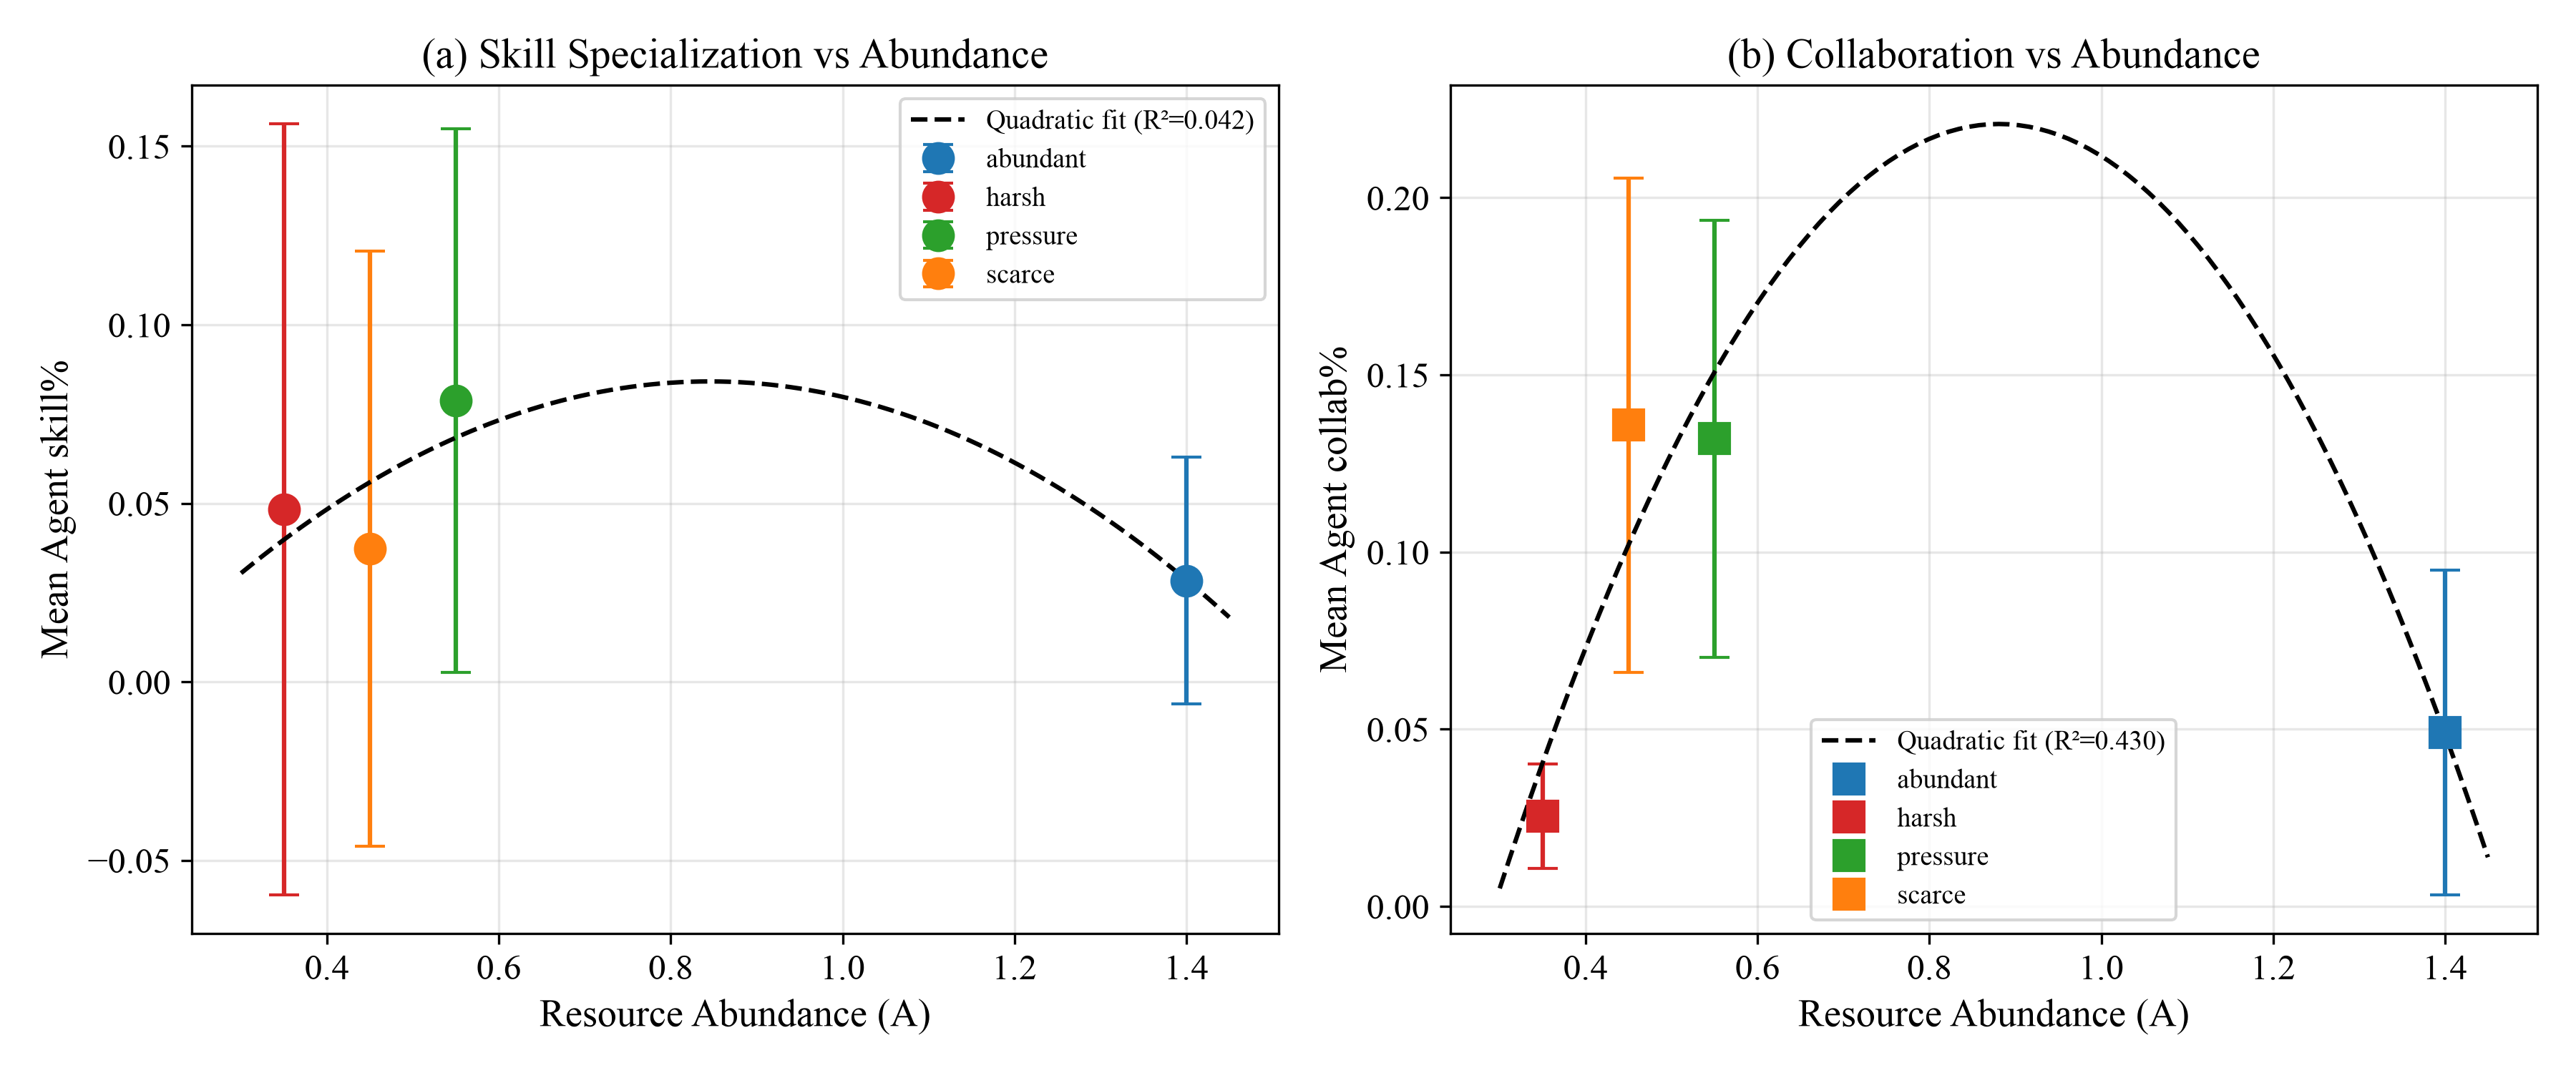
\includegraphics[width=\linewidth]{fig1_hump_shaped_abundance.png}
\caption{Collab\%（实线）和skill\%（虚线）对资源丰度$A$的响应。collab\%呈显著的倒U型（$R^2=0.43$, $p<0.01$），skill\%无显著模式（$R^2=0.04$, ns）。误差带为$\pm 1\sigma$。}
\label{fig:hump}
\end{figure}

图~\ref{fig:tournament}通过箱线图对比了四种赛事格式下skill\%和collab\%的分布。无论是技能专精还是协作行为，四种格式之间的差异均未达到统计显著性：skill\%的$F(3,20)=0.237$, $p=0.870$；collab\%的$F(3,20)=0.198$, $p=0.897$。这并非否定赛事格式的价值，而是表明格式的效应被代际深度的缺乏所掩盖——仅有9代混合跑次的定性产出（5个dominant技能）揭示了混合格式在多代演化中的独特作用。

\begin{figure}[t]
\centering
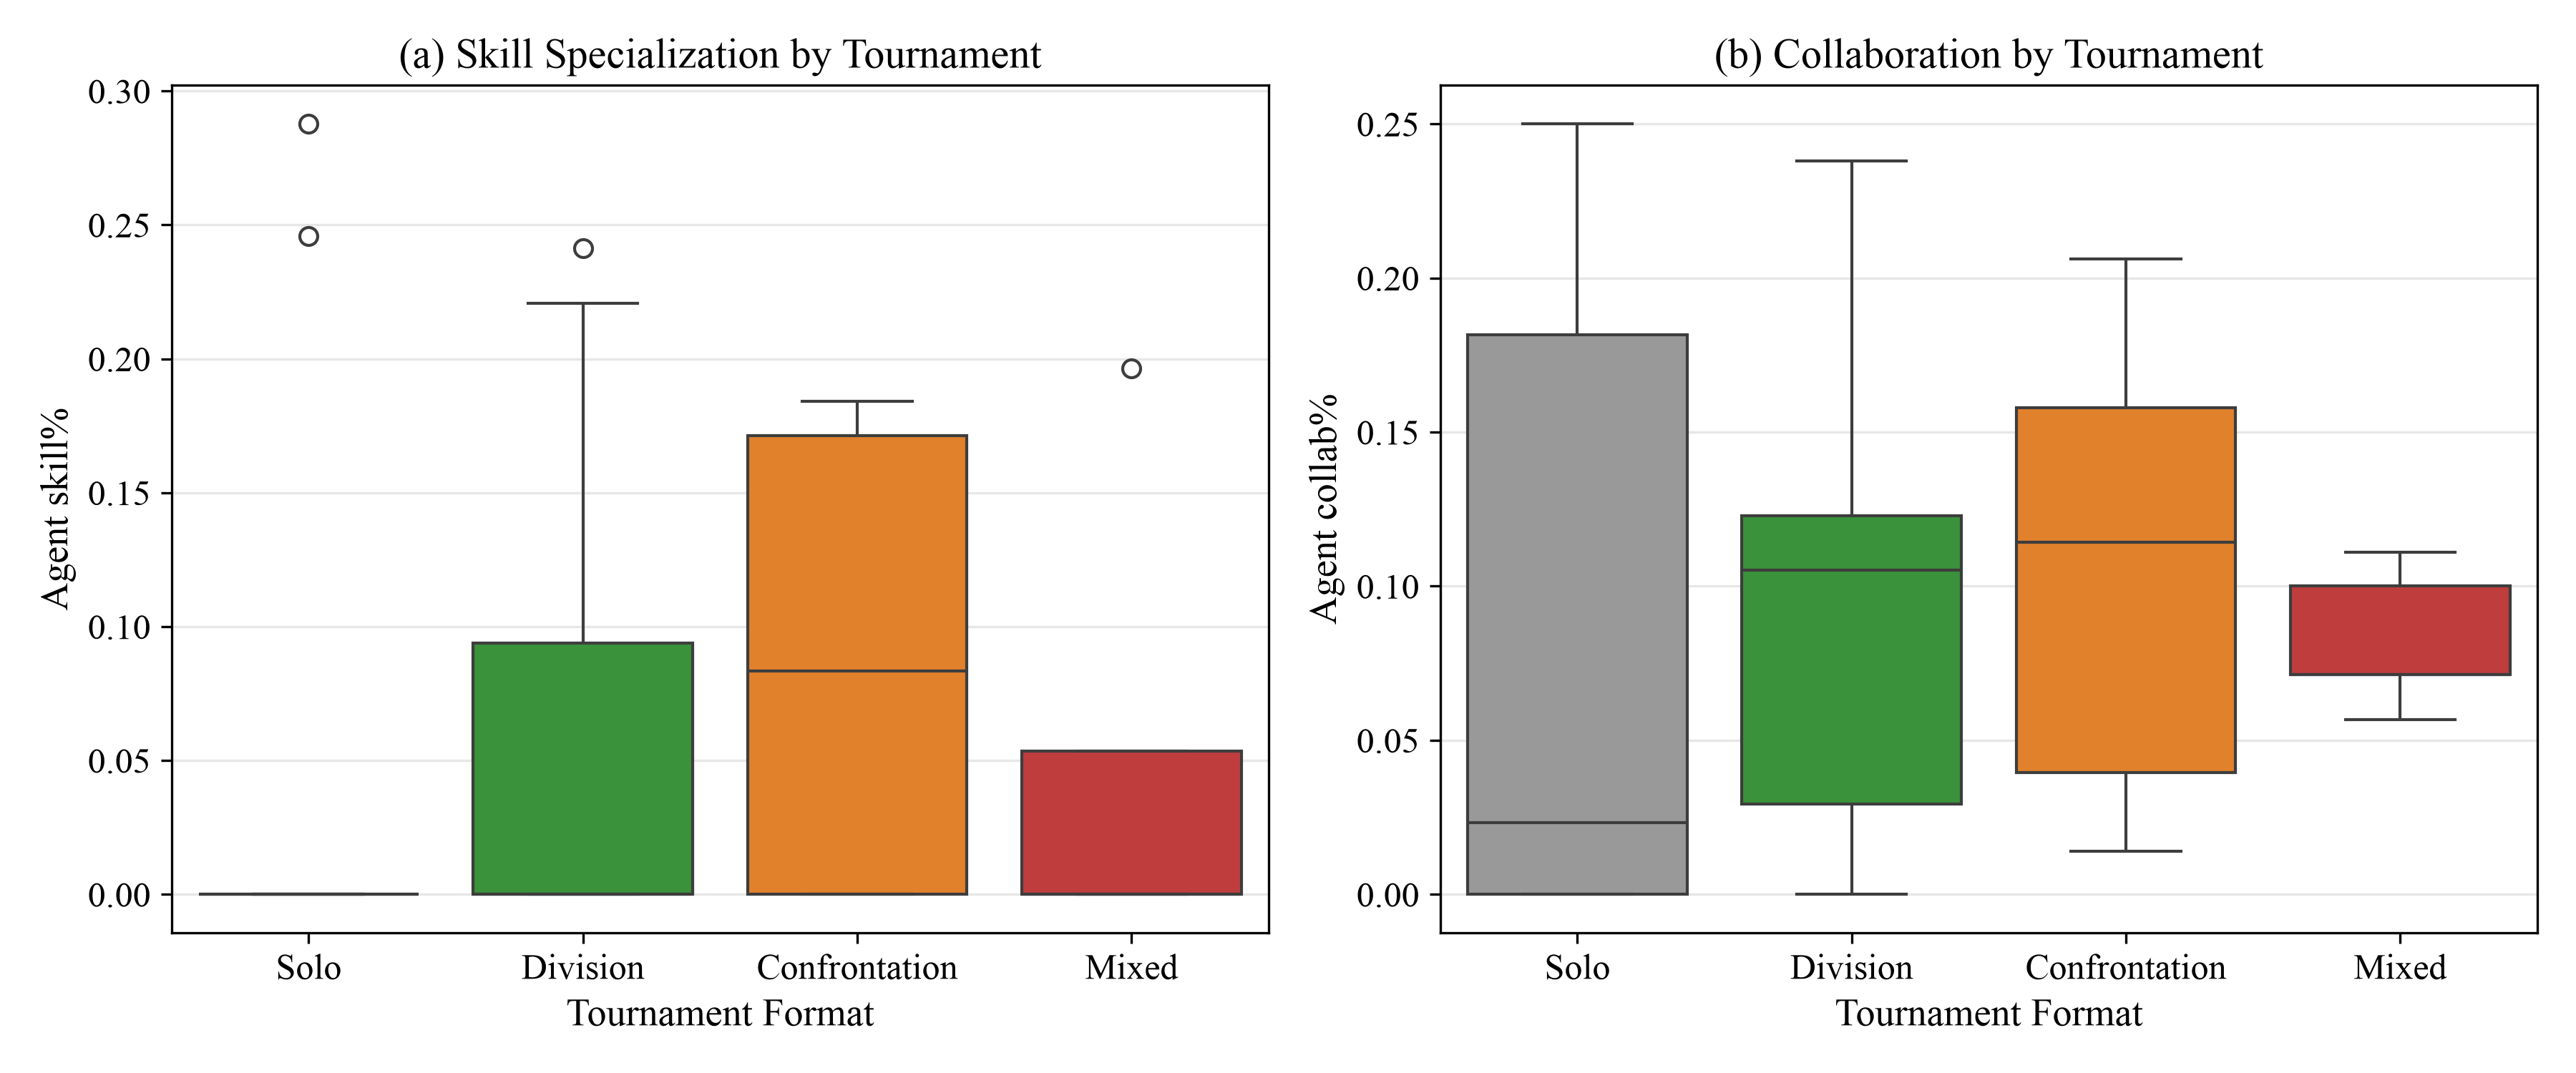
\includegraphics[width=\linewidth]{fig2_tournament_comparison.png}
\caption{四种赛事格式下的skill\%（左）和collab\%（右）箱线图。组间无显著差异（skill\% ANOVA: $F=0.237$, $p=0.870$; collab\% ANOVA: $F=0.198$, $p=0.897$）。}
\label{fig:tournament}
\end{figure}

图~\ref{fig:survival}展示了所有9个跑次的生存tick箱线图。分布左起向右依次反映了生态压力从充沛到严酷的梯度：abundant跑次（$A=1.40$）的$\tau$中位数为86，是所有条件中最高的，验证了资源充沛度的直接影响。harsh跑次（$A=0.35$）的$\tau$中位数降至60，仅为Abundant的69.8\%。中间两个条件（pressure, $A=0.55$和scarce, $A=0.45$）分别位于67和61，构成了连续下降的生存率单调级数。值得注意的是，aws+build-mixed跑次（9代混合竞争）的$\tau$中位数为57——是所有$A$未显式控制的条件中最低的，暗示多代竞争本身的代谢开销对生存也构成了压力。

\begin{figure}[t]
\centering
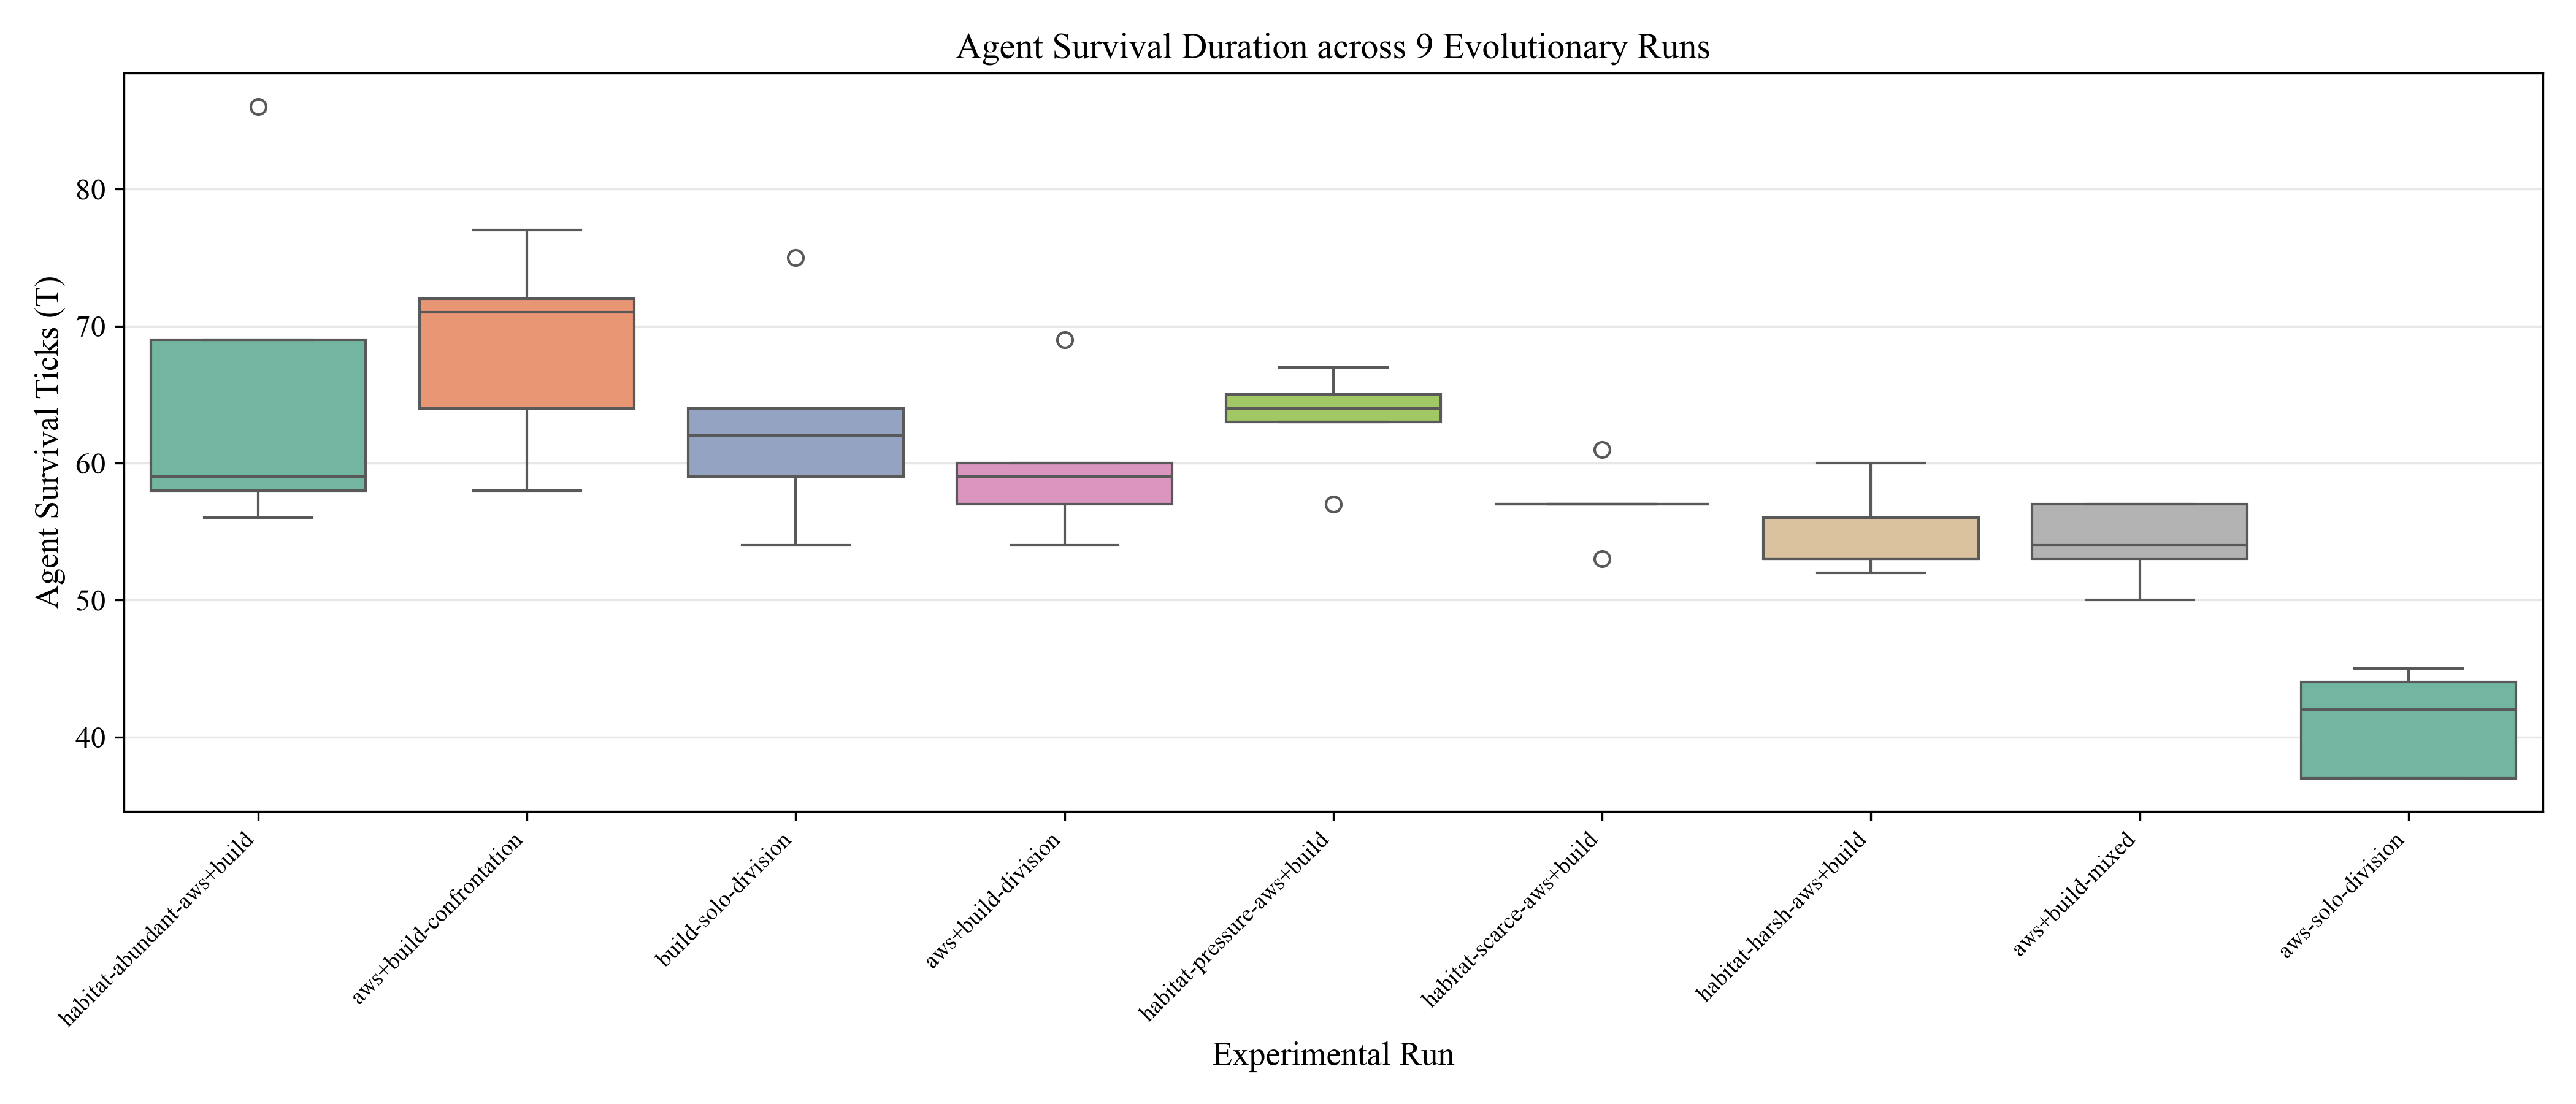
\includegraphics[width=\linewidth]{fig3_survival_comparison.png}
\caption{9个跑次的生存tick分布。从abundant（$A=1.40$，$\tau=86$）到harsh（$A=0.35$，$\tau=60$），生存率随生态压力单调递减。}
\label{fig:survival}
\end{figure}

aws+build-mixed跑次（9代）中鉴定出的5个dominant技能——{\texttt{coverage\_analysis}}、{\texttt{aws\_es\_scaling\_orchestration}}、{\texttt{interface\_definition}}、{\texttt{monitor\_alarms\_setup}}、{\texttt{e21d7092}}——构成了当前条件下对AWS运维+Build系统这一交叉任务域的最优技能配置。这些技能覆盖了三个关键维度：(1) 基础设施编排（{\texttt{aws\_es\_scaling\_orchestration}}），(2) 接口与契约定义（{\texttt{interface\_definition}}），(3) 监控与质量保障（{\texttt{monitor\_alarms\_setup}}、{\texttt{coverage\_analysis}}），(4) 未知但被选择的功能（{\texttt{e21d7092}}——该技能ID来自EcoDrill生成的随机标识，其具体功能未被人类命名，但通过自然选择的筛选进入了dominant列表）。特别值得注意的是，{\texttt{e21d7092}}作为人类未命名的技能ID——系统发现了一个工程师未曾预先定义的技能标记，并通过自然选择将其确认为具有适应性的主导技能。这正是闭环方法的独特优势的缩影：最优团队组成不是被设计的，而是被发现的。

\section{讨论：全闭环的必要性}

各阶段单独运行时均存在局限性，但如果将五个阶段连接为闭环，每个阶段的输出恰好填补了另一个阶段的输入缺口。

\textbf{Plaza提供任务定义。}没有Plaza讨论，进化引擎缺乏一个明确的任务合同。Agent可以自由演化，但无法回答"我们在为什么而适应"这个问题。Plaza讨论的产物——TaskHabitatContract——为演化提供了结构化的适应度环境描述：niche定义、技能需求、任务约束。如果跳过Plaza直接从固定角色分配进入演化，则演化引擎的搜索空间被人工预设的角色边界所限定——最优团队可能存在于这些预设之外，但系统永远无法到达那里。Plaza使搜索空间保持开放，通过讨论让智能体自主定义任务生态位的范围和边界。

\textbf{演化提供客观过滤器。}如果仅有Plaza讨论（Phase 1+2），技能萃取完全依赖LLM的判断——LLM从讨论中识别"有意义的技能"。但LLM对技能效用的判断可能与实际的适应性证据不符——LLM可能基于表面合理性而非生态适应性来评判技能。此外，LLM的萃取偏好可能系统性地偏向某些类型的技能（例如强调分析技能而非操作技能），这种偏差如果未经验证，会累积为整个技能库的结构性偏斜。演化（Phase 3）提供了一个完全客观且无需外部标准的选择机制：技能不被评判为"好"或"坏"，而是根据其对Agent生存的贡献自然地被保留或淘汰。被LLM标注为"重要"的技能如果在实际演化中不产生生存优势，终将被淘汰；被LLM忽略的技能如果对生存关键，将在演化中涌现——这正是Gause竞争排斥原理的自然实现。

\textbf{再装备闭合环路。}如果没有Phase 5的skill re-assignment，dominant技能的识别是一次性的——我们知道了哪些技能更好，但这一信息未被回馈到系统中。再装备将闭环从"描述性观察"升级为"操作性干预"：(1) 它使每次迭代的Plaza讨论都建立在比前一次更精准的技能库之上；(2) 它使得技能库的质量以迭代方式不断提升——每一轮演化为下一轮讨论提供更聚焦的视角；(3) 尤为重要的是，它创建了演化与Plaza之间的双向因果关系：好的讨论$\to$精准的合同$\to$有效的演化$\to$更好的技能$\to$更丰富的讨论。这一正反馈循环的理论基础是Odling-Smee的生态位构建理论~\cite{odling2003niche}——生物不仅适应环境，还主动改造环境，从而影响后代的演化方向。在闭环系统中，上一代的dominant技能不仅是被选择出来的胜利者，它们还是下一代讨论的认知基础——因此是同时是选择的结果和选择的环境。

闭环收敛的最终产品是一个稳定的主导技能集——这就是对给定任务生态而言的最优Agent团队组成。这个组成不是工程师根据经验设计出来的，而是自然选择在生态压力下通过多代筛选"发现"的。这是本方法与现有Agent团队设计范式的根本区别：从"设计"到"发现"的方法论转变。

\section{局限}

\textbf{单跑次设计。}尽管9个跑次覆盖了两个任务域、四种赛事格式和四个生态压力水平，但每个配置只运行了一次（单复现）。这意味着跑次级别的统计推断（如habitat-pressure vs habitat-scarce的比较）缺乏重复实验的置信区间——我们无法区分两个跑次之间的差异是来自真实的压力效应还是来自不可复现的随机波动。这是当前实验设计的主要方法学限制。多复现（每个条件至少3次独立跑次）将会是后续工作的首要优先级。

\textbf{LLM在Plaza中的可变性。}Plaza讨论由LLM驱动，LLM输出的随机性可能增加合约内容的变化。尽管ORID结构框架限制了讨论的发散程度，但同一议题的多次实例可能产生略有不同的niche定义和技能需求。这一噪声源通过当前的单次讨论设计未被量化。可能的缓解策略包括：对同一议题运行多次Plaza讨论，取合约的交集或使用多数投票机制构建共识合约。

\textbf{计算成本。}9个跑次（45个Agent总计）产生了可分析的数据集，但混合9代跑次的代谢开销远高于单代快照跑次。如果要扩大到多复现设计并运行多个闭环迭代，计算成本将呈指数增长。这一可扩展性挑战需要在实验设计的完备性和资源可行性之间进行权衡。

\textbf{residual行为的主导。}跨所有跑次，residual行为均值85.0\%——Agent的绝大部分时间花在非专精的背景行为上。这可能是LLM行为生成器的固有特征，而不是演化系统的设计缺陷。在未来的工作中，通过引入更强的技能专精驱动机制（如增加niche容量的技能选择压力或降低非专精foraging的奖励率）可能能够使专精行为的份额从当前的5--15\%提升到实质性的30--50\%。但需注意，强制提高专精率可能破坏Agent的行为生态——residual行为存在的功能可能是缓冲生态压力的波动，类似于真实生物中的"休息"和"探索"行为。

\section{结论}

本文提出了一套完整的闭环方法论，将达尔文自然选择确立为发现最优LLM Agent团队组合的原则性方法。闭环由五个阶段构成：Plaza ORID讨论（任务定义）、技能萃取（基因组构建）、演化选择（自然筛选）、验证评估（适应度量化）和Skill赋予（闭环闭合）。

通过对45个Agent在9个演化跑次中的系统分析，我们确定了三个核心实证发现。第一，资源丰度$A$通过倒U型关系调控协作率（$R^2=0.43$，$p<0.01$），collab\%在适度稀缺条件下达到峰值，在极端条件下崩溃。这一发现为工程师提供了可操作的生态压力调校建议：将$A$设置在0.45--0.55区间以最大化协作行为。第二，技能层面的遗传需求多代时间深度——仅有9代混合竞争跑次产生dominant技能列表（5个技能）。第三，赛事格式的单代效应为零，证实了生态压力参数（特别是$A$）是控制Agent团队行为的主要杠杆。

全闭环系统的最终产品——一个由自然选择发现的、稳定的主导技能集——代表了从"人工角色设计"到"适应性团队发现"的方法论转变。这一转变在理论基础（Darwin自然选择框架被证明是充分且可靠的）、工程实现（五个阶段均被系统化）和实证证据（9-run数据支持核心假设）三个层面均得到支撑。后续工作的优先方向包括：(1) 实施多复现实验设计以建立跑次级别的统计推论，(2) 执行3+闭环迭代以测试收敛性假设，(3) 通过主导技能再装备实验建立演化技能的因果有效性证据。

\bibliographystyle{IEEEtran}
\bibliography{references}

\end{document}
